\hfil
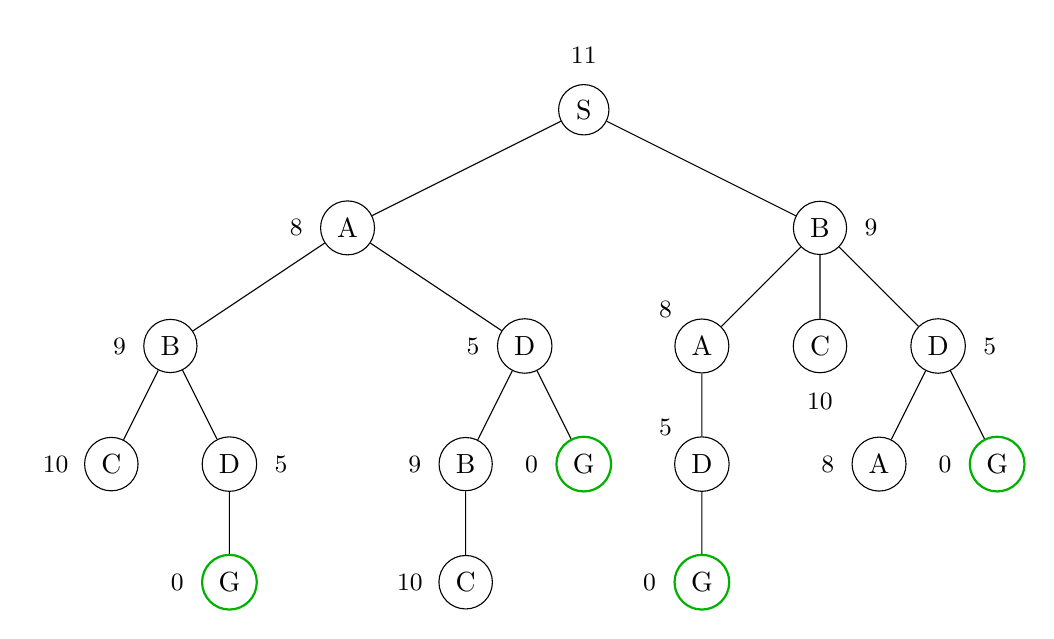
\begin{tikzpicture}[
    every node/.style = {shape=circle, draw, align=center}
    ]
    \node[label={\small 11}] {S}
    child { node[label=left:{\small 8}] {A} 
        child { node[label=left:{\small 9}] {B} 
            child { node[label=left:{\small 10}] {C} }
            child { node[label=right:{\small 5}] {D} 
                child { node[draw=black!30!green, thick, label=left:{\small 0}]  {G} }
            }
        }
        child [missing]
        child [missing]
        child { node[label=left:{\small 5}] {D} 
            child { node[label=left:{\small 9}] {B} 
                child { node[label=left:{\small 10}] {C} }
            }
            child { node[draw=black!30!green, thick, label=left:{\small 0}] {G} }
        }
    }
    child [missing]
    child [missing]
    child [missing]
    child { node[label=right:{\small 9}] {B} 
        child { node[label=above left:{\small 8}] {A} 
            child { node[label=above left:{\small 5}]  {D} 
                    child { node[draw=black!30!green, thick, label=left:{\small 0}]  {G} }
            }
        }
        child { node[label=below:{\small 10}] {C} }
        child { node[label=right:{\small 5}] {D} 
            child { node[label=left:{\small 8}] {A} }
            child { node[draw=black!30!green, thick, label=left:{\small 0}]  {G} }
        }
    };
\end{tikzpicture}

  